\documentclass[crop,class=article]{standalone}
%----------------------------Preamble-------------------------------%
\usepackage{tikz}                       % Drawing/graphing tools.
\usetikzlibrary{arrows.meta}            % Latex and Stealth arrows.
%--------------------------Main Document----------------------------%
\begin{document}
    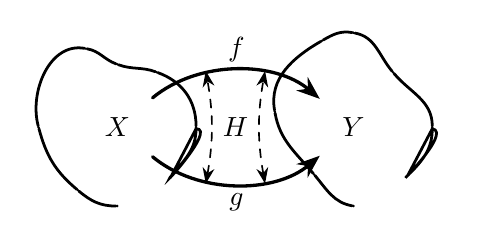
\begin{tikzpicture}[%
        line width=1pt,
        line cap=round,>={Stealth[black]},
        every edge/.style={draw=black,very thick},
        smalldot/.style={
            circle,
            fill=black,
            inner sep=0pt,
            outer sep=0
        }
    ]
        \begin{scope}[every node/.style=smalldot]
            % Set points defining the leftmost blob.
            \node at (0,0) (a) {};
            \node at (-0.5,0.2) (b) {};
            \node at (-1,1) (c) {};
            \node at (-0.4,2) (d) {};
            \node at (0, 1.8) (e) {};
            \node at (0.5, 1.7) (f) {};
            \node at (1,1) (g) {};
            \node at (0.7,0.4) (h) {};

            % Set points defining the rightmost blob.
            \node at (3,0) (a1) {};
            \node at (2.5,0.4) (b1) {};
            \node at (2,1.2) (c1) {};
            \node at (2.6,2.1) (d1) {};
            \node at (3, 2.2) (e1) {};
            \node at (3.5, 1.7) (f1) {};
            \node at (4,1) (g1) {};
            \node at (3.7,0.4) (h1) {};
        \end{scope}

        % Labels for the blobs X and Y.
        \node at (0,1) (i) {$X$};
        \node at (3,1) (i1) {$Y$};

        % Node indicating this is a homotopy.
        \node at (1.5,1) (ho) {$H$};

        % Nodes for drawing arrows between curves.
        \node at (1.1,0.15) (t1) {};
        \node at (1.1,1.85) (t2) {};
        \node at (1.9,0.15) (t3) {};
        \node at (1.9,1.85) (t4) {};

        % Draw a Hobby curve creating leftmost blob.
        \draw (a) to [out=180,in=-40] (b)
                  to [out=140,in=-75] (c)
                  to [out=105,in=170] (d)
                  to [out=-10,in=160] (e)
                  to [out=-20,in=160] (f)
                  to [out=-20,in=90] (g)
                  to [out=-90,in=50] (h)
                  to [out=-130,in=0] cycle;

        % Draw Hobby curve creating rightmost blob.
        \draw (a1) to [out=170,in=-50] (b1)
                   to [out=130,in=-80] (c1)
                   to [out=100,in=-150] (d1)
                   to [out=30,in=170] (e1)
                   to [out=-10,in=130] (f1)
                   to [out=-50,in=90] (g1)
                   to [out=-90,in=45] (h1)
                   to [out=-135,in=-10] cycle;

        % Draw arrows representing f and g.
        \path[shorten >=0.2cm,shorten <=0.2cm,->]
            (i) edge[bend left=40] node[above] {$f$} (i1);
        \path[shorten >=0.2cm,shorten <=0.2cm,->]
            (i) edge[bend right=40] node[below] {$g$} (i1);

        % Draw first arrow connecting f and g.
        \path[draw=black,dashed,<->]
            (t1) edge[bend right =10,semithick] (t2);

        % Draw second arrow connecting f and g.
        \path[draw=black,dashed,<->]
            (t3) edge[bend left =10,semithick] (t4);
    \end{tikzpicture}
\end{document}